\documentclass[11pt]{article}
\usepackage[a4paper,margin=2.3cm]{geometry}
\usepackage[T1]{fontenc}
\usepackage{lmodern,textcomp}
\usepackage{amsmath,amssymb,booktabs,graphicx,xcolor,caption}
\usepackage[colorlinks,linkcolor=blue!50!black,citecolor=blue!50!black,urlcolor=blue!50!black]{hyperref}
\captionsetup{font=small,labelfont=bf}
\newcommand{\thecov}{\texttt{thecov}}
\newcommand{\hk}{\,h\,\mathrm{Mpc}^{-1}}
\newcommand{\Chat}{\hat{C}}
\title{Validating \thecov's Gaussian covariance against DESI DR2 mocks:\\ LRG1 and QSO, fibre assignment, bin width and the structure of the excess}
\author{Validation note, branch \texttt{thecov2}}
\date{October 2026}
\begin{document}
\maketitle

\begin{abstract}
We compare the windowed Gaussian covariance computed by \thecov\ with the sample covariance of DESI DR2 mock power spectrum multipoles $P_{0,2,4}(k)$, for $0.02\le k\le 0.3\hk$ in $\Delta k = 0.005\hk$ bins, using 859 holi v3 altmtl realisations (LRG1 and QSO) and 25 AbacusSummit realisations available both with and without fibre assignment (\emph{complete} and \emph{altmtl}). For QSO, \thecov\ agrees with the mocks to $\lesssim 1\%$ in $\langle\chi^2\rangle/n$. For LRG1 the mocks show $\langle\chi^2\rangle/n \simeq 1.10$ (holi) and $1.10$--$1.17$ (Abacus). Four results organise this excess.
(i) Fibre assignment is not responsible: on identical Abacus realisations, altmtl and complete agree to $\Delta\langle\chi^2\rangle/n = 0.000$--$0.023 \pm 0.014$.
(ii) Changing the bin width separates a component of the excess that does not depend on $\Delta k$ (``Gaussian-like'', $a\simeq 0.10$ for LRG1 $P_0$ and $P_2$, $\simeq0$ for QSO) from one proportional to $\Delta k$ (non-Gaussian, $b$ growing from $0.02$ to $0.15$ per $0.005\hk$ in $P_0$).
(iii) Per-object weight scatter, $\langle w^2\rangle\neq\langle w\rangle^2$, is handled correctly by a smoothed window $m(\mathbf{x})$; the naive window would have hidden part of the excess.
(iv) The excess is concentrated in a few directions of data space: the leading one is a broad-band $P_0$ amplitude/dilation mode whose variance is $\simeq 6$ times \thecov's, the second a $P_2$ amplitude mode. With a few nuisance parameters marginalised, \thecov\ underestimates the variance of an amplitude-like parameter by $15$--$25\%$ and that of a quadrupole amplitude by $\simeq70\%$ for LRG1 at $k_{\max}=0.2\hk$ (more at $0.3$). The per-mock estimator normalisation explains only $\simeq 2\%$ of the amplitude scatter, so the isotropic local-average effect is small; the amplitude modes point to super-sample (including tidal) and connected non-Gaussian terms that \thecov\ does not contain.
\end{abstract}

\tableofcontents

%======================================================================
\section{Set-up}
\label{sec:setup}

\paragraph{Mocks and spectra.} Power spectrum multipoles are those of the DESI DR2 full-shape pipeline (\texttt{jaxpower}), read from the \texttt{summary\_statistics/full\_shape/base} directory for three mock families:
\begin{itemize}
\item \textbf{holi v3 altmtl}: 859 realisations, LRG1 ($0.4<z<0.6$) and QSO ($0.8<z<2.1$), NGC, SGC and GCcomb;
\item \textbf{AbacusSummit 2nd gen.\ DR2 complete} and \textbf{altmtl}: the same 25 realisations without and with fibre assignment, LRG1.
\end{itemize}
We use $0.02\le k\le0.3\hk$ in $\Delta k=0.005\hk$ bins ($n=3\times56=168$ data points), and the coarser binnings $\Delta k=0.01$ and $0.02\hk$ (Sec.~\ref{sec:binwidth}). The window (randoms, weights) is taken from one realisation per family (holi mock 173, Abacus mock 0), with one random file.

\paragraph{Covariance.} \thecov\ computes the windowed Gaussian covariance in configuration space from pair counts of randoms carrying the clustering window $W=m^2$ and the shot-noise window $S=\bar n\langle w^2\rangle$, where
\begin{equation}
m(\mathbf{x}) = \bar n(\mathbf{x})\,\langle w\rangle(\mathbf{x}) = \mathrm{E}\Big[\textstyle\sum_g w_g\,\delta_D(\mathbf{x}-\mathbf{x}_g)\Big]
\end{equation}
is the mean weighted density, $w=\texttt{WEIGHT}\times\texttt{WEIGHT\_FKP}$. Three constructions of $m$ at each random are compared: \emph{smoothed} ($\alpha\,\rho_r(z)$ times the mean weight of the 32 nearest randoms; the default), \emph{nx} ($\texttt{NX}\times\texttt{WEIGHT\_FKP}$, no smoothing), and \emph{naive} (each random's own weight). The model power spectrum is the mock mean rescaled by $\mathrm{norm}/\!\int m^2$ (Sec.~\ref{sec:corrections}). GCcomb is the norm-weighted mean of NGC and SGC in the files (to $5\times10^{-14}$), so its covariance is the corresponding combination of the cap covariances.

\paragraph{Statistics.} With $N$ mocks, $\langle\chi^2\rangle/n$ is the mean of $(\hat{\mathbf P}_i-\bar{\mathbf P})^{\rm T}C^{-1}(\hat{\mathbf P}_i-\bar{\mathbf P})/[n(1-1/N)]$, expected to be $1\pm\sqrt{2/(nN)}$ ($\pm0.004$ for holi, $\pm0.022$ for Abacus). We also use the per-element variance ratio $\sigma^2_{\rm mock}/\sigma^2_{\rm thecov}$, the eigenvalues of the whitened mock covariance $E=C^{-1/2}\Chat C^{-1/2}$ against the Marchenko--Pastur (MP) range, and variances along chosen directions.

%======================================================================
\section{Corrections required to compare with the DESI files}
\label{sec:corrections}

Before any physics, four conventions had to be matched. Together they moved the variance ratio from $0.77$ to $\simeq1.1$.
\begin{enumerate}
\item \textbf{Model normalisation.} \texttt{jaxpower} normalises by $\mathrm{norm}=\alpha\sum_c D_cR_c/V_c$ on $10\,h^{-1}$Mpc cells, which smooths over the fine veto masks. Its mean $\hat P$ is therefore $(\int m^2/\mathrm{norm})\times$ the windowed $P$. We find $\int m^2/\mathrm{norm}=1.22$ (LRG1, holi), $1.11$ (QSO), $1.15$--$1.18$ (LRG1, Abacus). Feeding the raw mock mean to \thecov\ inflates the clustering terms by $(1.22)^2\simeq1.5$; the model must be $\bar P\times\mathrm{norm}/\!\int m^2$.
\item \textbf{Shot noise.} The files subtract the realised shot noise, $\texttt{num\_shotnoise}/\mathrm{norm}$. Its catalogue estimate $\sum_d w^2+\alpha^2\sum_r w^2$ from a single random file is $16$--$19\%$ too high (LRG1) because the spectra used many more randoms. We normalise the shot-noise window to the files' mean \texttt{num\_shotnoise}.
\item \textbf{GCcomb} is combined from the caps exactly, as above.
\item \textbf{$k_{\min}=0.02\hk$.} The first bins ($kL\lesssim1$) are outside the validity of any local windowed Gaussian covariance and make it non-positive-definite.
\end{enumerate}

%======================================================================
\section{Summary of the comparison}
\label{sec:summary}

\begin{table}[h]
\centering\small
\begin{tabular}{lll cccccc}
\toprule
mocks & bin & region & smoothed & nx & naive & $\Delta k\times2$ & $\Delta k\times4$ & $\pm$\\
\midrule
holi & LRG1 & NGC & 1.096 & 1.112 & 1.031 & 1.120 & 1.204 & 0.004\\
holi & LRG1 & SGC & 1.099 & 1.114 & 1.067 & 1.123 & 1.190 & 0.004\\
holi & LRG1 & GCcomb & 1.098 & 1.110 & -- & 1.123 & 1.199 & 0.004\\
holi & QSO & NGC & 1.009 & 1.005 & 0.993 & 1.024 & 1.062 & 0.004\\
holi & QSO & SGC & 1.000 & 1.001 & 0.990 & 1.013 & 1.043 & 0.004\\
holi & QSO & GCcomb & 1.004 & 1.001 & -- & 1.016 & 1.053 & 0.004\\
Ab.\ compl. & LRG1 & NGC & 1.127 & 1.128 & 1.119 & 1.100 & 1.184 & 0.022\\
Ab.\ compl. & LRG1 & SGC & 1.121 & 1.117 & 1.123 & 1.149 & 1.210 & 0.022\\
Ab.\ compl. & LRG1 & GCcomb & 1.174 & 1.173 & -- & 1.184 & 1.268 & 0.022\\
Ab.\ altmtl & LRG1 & NGC & 1.104 & 1.131 & 1.054 & 1.082 & 1.120 & 0.022\\
Ab.\ altmtl & LRG1 & SGC & 1.121 & 1.092 & 1.144 & 1.114 & 1.175 & 0.022\\
Ab.\ altmtl & LRG1 & GCcomb & 1.157 & 1.166 & -- & 1.162 & 1.211 & 0.022\\
\bottomrule
\end{tabular}
\caption{$\langle\chi^2\rangle/n$ for $0.02\le k\le0.3\hk$, $P_{0,2,4}$, with the three constructions of $m$ (Sec.~\ref{sec:setup}) at $\Delta k=0.005\hk$, and with the smoothed $m$ at $\Delta k=0.01$ and $0.02\hk$. The last column is the statistical error at $\Delta k=0.005$; it grows as $\sqrt{2}$ and $2$ for the coarser binnings.}
\label{tab:chi2}
\end{table}

QSO is consistent with \thecov\ at $\Delta k=0.005$; at $\Delta k=0.02$ it rises to $1.04$--$1.06$, a non-Gaussian high-$k$ tail (Sec.~\ref{sec:binwidth}). LRG1 is not: $\langle\chi^2\rangle/n=1.10$ in holi, the same with nx and smoothed windows, and it grows with the bin width. QSO's covariance is dominated by shot noise ($\bar nP<1$), so it checks the shot-noise terms, the normalisation and the model correction; the LRG1 excess is in the clustering terms.

%======================================================================
\section{Weights: why $m$ must be smoothed}
\label{sec:weights}

The clustering terms of the Gaussian covariance contain two factors of $m$ at (nearly) the same point. Pairs of randoms weighted by their own weights give $w_iw_j$, i.e.\ one factor of $m$ at each end of the pair, which is the window of $\langle\hat P\rangle$, not of its covariance. Each end must carry an unbiased estimate of $m^2$, and a single object cannot provide one: its own weight squared has expectation $\langle w^2\rangle$, larger than $\langle w\rangle^2$ by $1+\mathrm{var}(w)/\langle w\rangle^2$. The second factor must come from neighbours, i.e.\ from a smoothed $m$. This is exact for stochastic weights that are independent between objects and of the density field: the clustering windows involve $\langle w\rangle$, the shot-noise windows $\langle w^2\rangle$ (each random's own $w^2$ estimates it without bias).

\begin{table}[h]
\centering\small
\begin{tabular}{lll ccc cc}
\toprule
 & & & & \multicolumn{2}{c}{$\int m^2/\mathrm{norm}$} & \multicolumn{2}{c}{$\langle\chi^2\rangle/n$}\\
mocks & bin & region & $\langle w^2\rangle/\langle w\rangle^2$ & smoothed & naive & smoothed & naive\\
\midrule
holi & LRG1 & NGC & 1.165 & 1.225 & 1.519 & 1.096 & 1.031\\
holi & LRG1 & SGC & 1.157 & 1.210 & 1.465 & 1.099 & 1.067\\
holi & QSO & NGC & 1.039 & 1.110 & 1.218 & 1.009 & 0.993\\
holi & QSO & SGC & 1.037 & 1.107 & 1.190 & 1.000 & 0.990\\
Ab.\ compl. & LRG1 & NGC & 1.000 & 1.177 & 1.179 & 1.127 & 1.119\\
Ab.\ compl. & LRG1 & SGC & 1.000 & 1.147 & 1.153 & 1.121 & 1.123\\
\bottomrule
\end{tabular}
\caption{Weight scatter of the data and its effect. The naive window overestimates $\int m^2$ by $\simeq\langle w^2\rangle/\langle w\rangle^2$, as predicted, and inflates the covariance. In Abacus complete the weights barely scatter and the two windows coincide.}
\label{tab:weights}
\end{table}

\begin{figure}[h]
\centering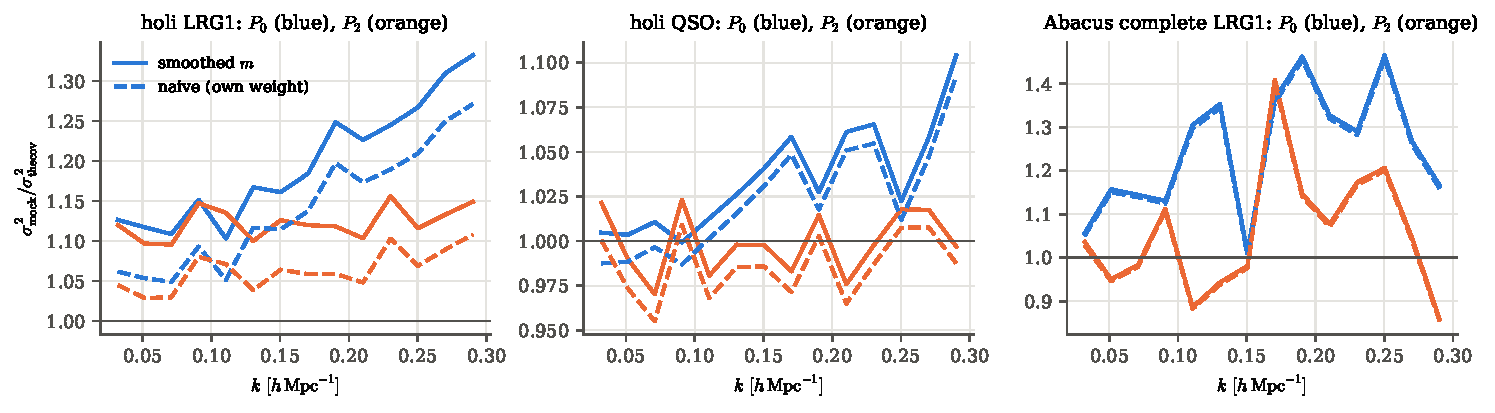
\includegraphics[width=\textwidth]{fig3_weights.pdf}
\caption{Variance ratio (mean over $0.02\hk$-wide groups of bins, both caps) with the smoothed and naive windows. The naive window adds a nearly flat $\simeq5$--$7\%$ to \thecov's LRG1 clustering variance and $\simeq2\%$ to QSO's. The weights in Abacus complete barely scatter and both constructions coincide (right), a null test.}
\label{fig:weights}
\end{figure}

Table~\ref{tab:weights} and Fig.~\ref{fig:weights} show the expected pattern: LRG1 weights scatter by $16\%$ (completeness weights from fibre assignment), QSO by $4\%$, Abacus complete by $0.05\%$. The naive window increases $\int m^2$ by the weight scatter and the covariance accordingly. Note the trap: with the naive window, LRG1 looks \emph{better} ($\langle\chi^2\rangle/n=1.03$ instead of $1.10$), because the overestimated window partly compensates the missing terms discussed below. The control (Abacus complete, $\langle w^2\rangle/\langle w\rangle^2=1.0005$) shows identical results for both, as it must.

%======================================================================
\section{Fibre assignment: Abacus altmtl versus complete}
\label{sec:fibre}

\begin{figure}[h]
\centering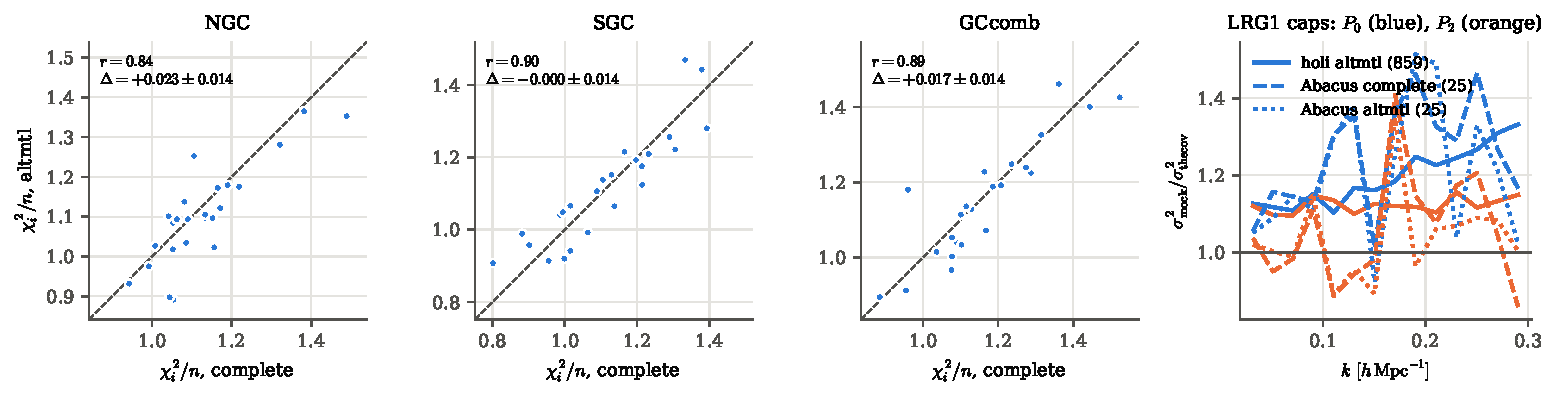
\includegraphics[width=\textwidth]{fig1_altmtl_complete.pdf}
\caption{Left three panels: $\chi^2_i/n$ of each Abacus realisation with fibre assignment (altmtl) against the same realisation without (complete); $r$ is the correlation coefficient and $\Delta$ the mean paired difference complete $-$ altmtl. Right: variance ratio of $P_0$ (blue) and $P_2$ (orange) for holi altmtl (859 mocks) and the two Abacus versions (25 mocks).}
\label{fig:fibre}
\end{figure}

Because the two Abacus versions share the underlying realisation, the per-mock $\chi^2_i$ are strongly correlated ($r=0.84$--$0.90$) and their difference is measured to $\pm0.014$ instead of the $\pm0.03$ of two independent sets. The differences, $+0.023\pm0.014$ (NGC), $0.000\pm0.014$ (SGC) and $+0.017\pm0.014$ (GCcomb), are consistent with zero, and the scale dependence of the variance ratio is the same with and without fibre assignment, and the same as in holi (Fig.~\ref{fig:fibre}, right). Fibre assignment adds at most $\simeq2\%$ to $\langle\chi^2\rangle/n$: the excess is not a consequence of the density-dependent selection or of the weights that compensate it, but is present in the complete mocks.

%======================================================================
\section{Bin width: Gaussian-like and non-Gaussian excess}
\label{sec:binwidth}

The Gaussian covariance of a bin scales as $1/N_{\rm modes}\propto1/\Delta k$, while connected non-Gaussian terms (trispectrum, super-sample) are smooth functions of $(k,k')$ and do not average down within a bin. Writing the per-element excess at bin width $f\times0.005\hk$ as
\begin{equation}
\frac{\sigma^2_{\rm mock}}{\sigma^2_{\rm thecov}}-1 = a(k) + b(k)\,f,
\label{eq:ab}
\end{equation}
$a$ collects anything with Gaussian scaling (a missing or mis-normalised Gaussian term) and $b$ the non-Gaussian variance in units of the Gaussian variance of a $0.005\hk$ bin. We fit Eq.~\eqref{eq:ab} to $f=1,2,4$ in $0.02\hk$-wide groups (errors from bootstrap over mocks).

\begin{figure}[t]
\centering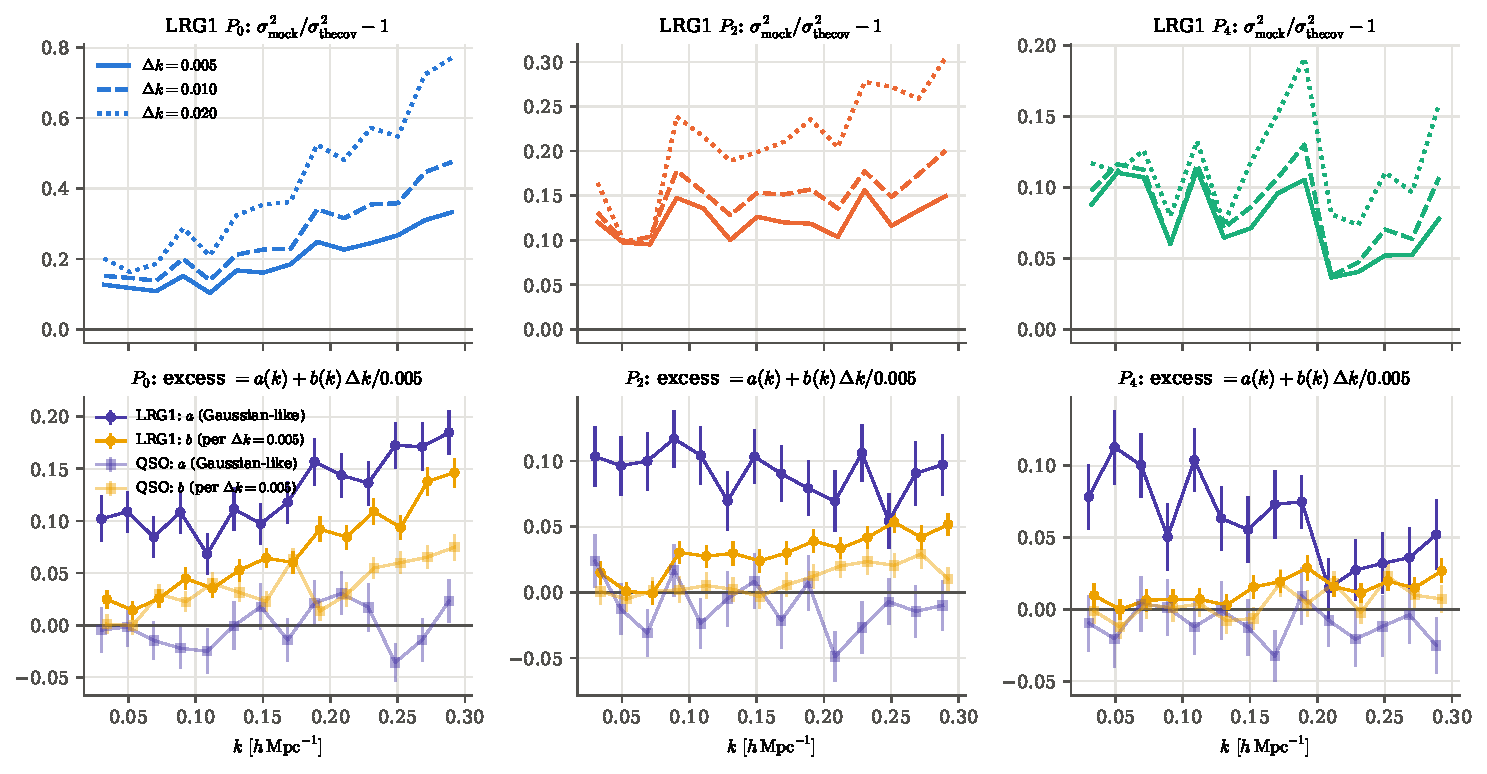
\includegraphics[width=\textwidth]{fig2_binwidth.pdf}
\caption{Top: LRG1 (holi, NGC and SGC averaged) excess variance for three bin widths. Bottom: the decomposition Eq.~\eqref{eq:ab} for LRG1 (dark) and QSO (light): $a$ (violet) does not depend on $\Delta k$, $b$ (yellow) is proportional to it.}
\label{fig:binwidth}
\end{figure}

Figure~\ref{fig:binwidth} shows:
\begin{itemize}
\item \textbf{Non-Gaussian part.} $b$ grows with $k$ and is largest in $P_0$: from $0.02$ at $k\simeq0.03$ to $0.15$ at $k\simeq0.29\hk$ for LRG1 ($0.05$ in $P_2$, $\lesssim0.03$ in $P_4$), and up to $0.07$ in QSO $P_0$. At $\Delta k=0.02\hk$ it is the dominant part of the excess at $k>0.15\hk$.
\item \textbf{Gaussian-like part.} For QSO, $a\simeq0$ at all $k$, as expected. For LRG1, however, $a\simeq0.10$ in $P_0$ and $P_2$ over the whole range (rising to $\simeq0.17$ in $P_0$ at $k>0.2$), and $0.05$--$0.10$ in $P_4$. It is also present in the Abacus mocks (mean $a_0\simeq0.14$--$0.18\pm0.03$ in complete and altmtl). This corrects an earlier estimate ($a\simeq0.025$) based on $\langle\chi^2\rangle/n$ of the full vector, which mixes the two parts.
\end{itemize}

The Gaussian-like $\simeq10\%$ is therefore specific to LRG1, independent of fibre assignment, and independent of the construction of $m$ at the scales probed by the smoothed, nx and patch windows. Two candidates remain, both of which affect the clustering terms only (hence not QSO):
\begin{enumerate}
\item \emph{Window structure below the smoothing scale.} An exact FFT-mesh Gaussian calculation with $m$ taken directly from random counts in cells (window ``B''), converged down to $1.5\,h^{-1}$Mpc, gave $6$--$9\%$ more $P_0$ variance than \thecov, and accounted for the low-$k$ excess (mocks/B $\simeq1.01$--$1.02$ at $k<0.05$). With \thecov's own $m$ the mesh calculation agrees with \thecov\ to $0.3\%$ (isotropic model). $W=m^2$ at a single point is itself a local approximation: near the many small veto holes and boundaries, $m(\mathbf{x})m(\mathbf{x}+\mathbf{r})\neq m^2(\mathbf{x})$ for $r$ within a correlation length.
\item \emph{The model normalisation.} The correction $\mathrm{norm}/\!\int m^2$ is a single number ($1/1.22$) applied at all $k$. The relevant quantity is the window pair count at separations $\sim10$--$100\,h^{-1}$Mpc, which need not coincide with the $10\,h^{-1}$Mpc-cell norm; a $5\%$ error in the effective model amplitude gives $10\%$ in the clustering variance. LRG1 has the largest $\int m^2/\mathrm{norm}$ of the samples considered, QSO the smallest.
\end{enumerate}
Both can be tested with existing machinery: pair counts of $m\otimes m$ at $10$--$100\,h^{-1}$Mpc against norm and $\int m^2$ (item 2), and window B extended to $k=0.3$ (item 1).

%======================================================================
\section{Directions in which the mocks and \thecov\ differ}
\label{sec:directions}

\begin{figure}[t]
\centering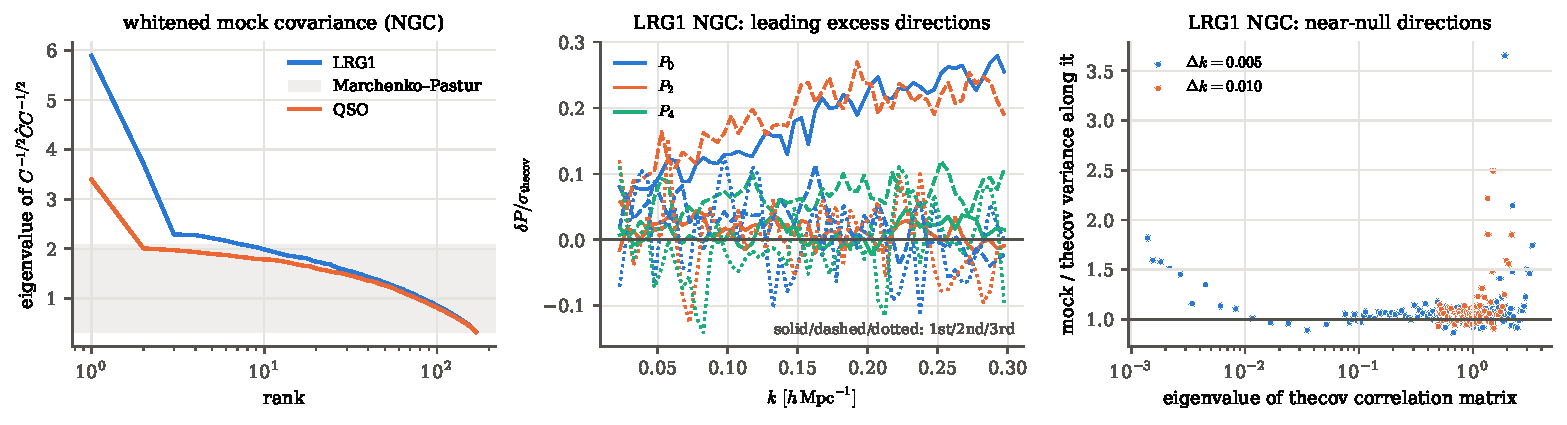
\includegraphics[width=\textwidth]{fig4_directions.pdf}
\caption{Left: eigenvalues of the whitened mock covariance $E=C^{-1/2}\Chat C^{-1/2}$ (holi NGC); grey: the MP range for $n=168$, $N=859$. Middle: the three leading excess directions for LRG1 NGC in data space, in units of \thecov's $\sigma$ per element. Right: variance ratio along each eigenvector of \thecov's correlation matrix against its eigenvalue, at $\Delta k=0.005$ and $0.01\hk$.}
\label{fig:directions}
\end{figure}

\paragraph{The excess is low-rank.} If \thecov\ were exact, the eigenvalues of $E$ would fill the MP range. For QSO only one eigenvalue (3.4) lies above it. For LRG1, the top two eigenvalues are $5.9$ and $3.7$, and the rest of the spectrum is shifted up uniformly by $\simeq10\%$, the Gaussian-like part $a$ of Sec.~\ref{sec:binwidth} (Fig.~\ref{fig:directions}, left).

\paragraph{What the leading directions are.} Whitened templates $u=C^{-1/2}t$ identify them. The \textbf{first} direction (eigenvalue 5.9) contains $95\%$ of the whitened $P_0{+}P_2{+}P_4$ amplitude template $t=\bar P$ and $91\%$ of the dilation template $t=-k\,\partial\bar P/\partial k$; the two are nearly degenerate once whitened. It is a smooth, broad-band $P_0$ mode growing with $k$ (Fig.~\ref{fig:directions}, middle). The \textbf{second} (3.7) contains $73\%$ of a $P_2$-only amplitude template. Along the amplitude template itself, the mocks have $5.6$ times \thecov's variance ($k\le0.3$); along the $P_2$ amplitude, $3.1$ times.

\paragraph{Near-null directions at fine binning.} At $\Delta k=0.005\hk$, adjacent bins are strongly correlated by the window, and \thecov's correlation matrix has eigenvalues down to $10^{-3}$. The corresponding eigenvectors are differences between neighbouring bins. Along them the mocks have $1.5$--$1.8$ times the predicted variance; at $\Delta k=0.01\hk$ the smallest eigenvalue is $0.5$ and the ratio is $\simeq1$ (Fig.~\ref{fig:directions}, right). These directions depend on the detailed shape of the window kernel, a Gaussian-level effect, and a smooth non-Gaussian term cancels in them. They contribute a few per cent to $\langle\chi^2\rangle/n$ at $\Delta k=0.005$ and are irrelevant for smooth parameter derivatives, but a goodness-of-fit $\chi^2$ will feel them.

%======================================================================
\section{Amplitude modes, super-sample covariance and the local-average effect}
\label{sec:ssc}

A long-wavelength mode $\delta_b$ larger than the survey changes the measured multipoles coherently: $\Delta\hat P_\ell(k)= [R_\ell(k)-2P_\ell(k)]\,\delta_b$ for an estimator normalised by the realised mean density, where $R_\ell$ is the physical response (growth, dilation, bias) and $-2P_\ell$ the local-average (LA) effect. In redshift space the long mode's own anisotropy (its Kaiser term and tidal components) adds responses that change $P_2$ (and $P_0$) without changing the mean density (Akitsu, Takada \& Li 2017; Wadekar \& Scoccimarro 2020). These terms produce exactly the kind of low-rank amplitude-like excess seen in Sec.~\ref{sec:directions}.

\begin{figure}[t]
\centering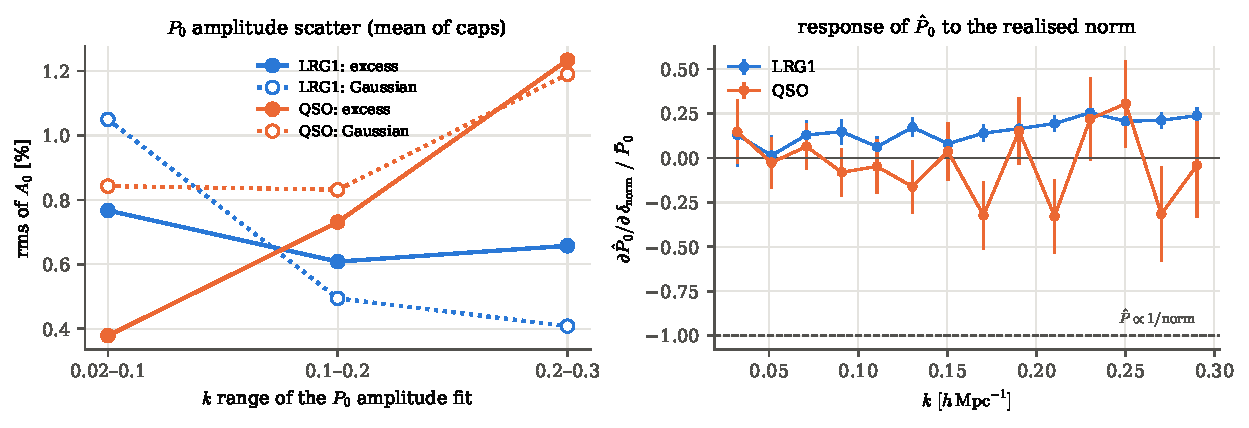
\includegraphics[width=0.85\textwidth]{fig5_amplitude.pdf}
\caption{Left: rms of the fitted $P_0$ amplitude $A_0$ (template $\bar P_0$) over three $k$ ranges: its excess over \thecov's prediction (solid) and the prediction itself (dotted), mean of the caps. Right: slope of $\hat P_0$ against the per-mock fluctuation of the estimator's normalisation, in units of $\bar P_0$, with standard regression errors.}
\label{fig:amplitude}
\end{figure}

\paragraph{The $k$-dependence separates SSC from the trispectrum.} We fit an amplitude to $P_0$ alone in three $k$ ranges (Fig.~\ref{fig:amplitude}, left). For LRG1 the excess amplitude scatter is nearly constant, $0.6$--$0.8\%$ (NGC: $0.67$, $0.51$, $0.58\%$; SGC: $0.86$, $0.70$, $0.74\%$), present already at $k<0.1\hk$: the signature of a super-sample response. For QSO it grows from $0.3$--$0.4\%$ at $k<0.1$ to $1.0$--$1.5\%$ at $k>0.2\hk$: the signature of the connected (and Poisson) trispectrum, with a weak super-sample part, consistent with QSO's much larger volume. The LRG1 $P_2$ amplitude has an excess of $3$--$5\%$ in every range, and is only weakly correlated with the $P_0$ amplitude ($r\simeq0.1$--$0.3$): two independent long-mode responses, as expected for isotropic and tidal super-sample modes.

\paragraph{The local-average response, measured.} \texttt{jaxpower}'s normalisation is computed for each mock from its own data and randoms, so the fluctuation $\delta_{\rm norm}=\mathrm{norm}_i/\langle\mathrm{norm}\rangle-1$ traces the survey-mean density of each realisation (plus Poisson noise). We find $\sigma(\delta_{\rm norm})=0.43\%$ (LRG1 NGC) and $0.75\%$ (SGC), against a Poisson expectation of $\simeq0.13$--$0.26\%$ and $0.18$--$0.36\%$, so most of it is clustering. Regressing $\hat P_0(k)$ on $\delta_{\rm norm}$ over the 859 mocks (Fig.~\ref{fig:amplitude}, right):
\begin{itemize}
\item the slope is positive and small, $\partial\hat P_0/\partial\delta_{\rm norm}\simeq(0.1\to0.25)\,\bar P_0$ rising with $k$, far from the $-\bar P_0$ that a pure rescaling $\hat P\propto1/\mathrm{norm}$ would give. If the realised norm scales as $(1+\delta_b)^2$ and $\hat P_0$ as $1+(R-2)\delta_b$, the slope is $(R-2)/2$ diluted by the Poisson part: the physical response and the local-average effect nearly cancel for the isotropic mode, with a residual growing with $k$ as the dilation term does;
\item the correlation of the fitted amplitude with $\delta_{\rm norm}$ is $0.14$ (NGC) and $0.17$ (SGC) for LRG1 and $0.00$--$0.02$ for QSO. The survey-mean density therefore explains only $\simeq2$--$3\%$ of the LRG1 amplitude variance; removing it from each mock changes $\langle\chi^2\rangle/n$ by $0.002$--$0.003$ and the excess amplitude scatter from $0.54$ to $0.54\%$ (NGC).
\end{itemize}
The isotropic, density-tracing super-sample mode with its local-average counterpart is thus a minor contributor. The large, $k$-independent $P_0$ and $P_2$ amplitude scatter of LRG1 must come from long modes that do not change the survey's mean density (tidal and redshift-space anisotropic components of the background, and, if the mock randoms take their redshifts from each mock's own data, the radial modes they absorb) or from a broad-band component of the trispectrum. A super-sample module for \thecov\ must therefore include the anisotropic responses in the redshift-space formalism of Wadekar \& Scoccimarro (2020) and model the local average for \texttt{jaxpower}'s realised normalisation; an isotropic $\sigma_b^2$ alone would underpredict it.

%======================================================================
\section{Impact on parameter errors}
\label{sec:params}

Since the excess is concentrated in amplitude-like directions, its impact on parameters depends on what is marginalised. We use four templates built from the mock mean: an overall amplitude $A$ (template $\bar P_\ell$, a proxy for $b\sigma_8$), a quadrupole amplitude $A_2$ ($\bar P_2$ only, a proxy for $f\sigma_8$), dilation $\alpha$ ($-k\,\partial\bar P_\ell/\partial k$) and a constant in $P_0$ (shot noise). For each mock we fit them by generalised least squares with \thecov's $C$ and compare the scatter of the estimates over the mocks with \thecov's prediction $(T^{\rm T}C^{-1}T)^{-1}$. A ratio of 1 means \thecov's errors are right; the statistical error on each ratio is $\simeq5\%$ for holi and $\simeq30\%$ for Abacus.

\begin{table}[h]
\centering\small
\begin{tabular}{llll ccc cccc}
\toprule
 & & & & \multicolumn{3}{c}{one parameter} & \multicolumn{4}{c}{jointly}\\
mocks & bin & region & $k_{\max}$ & $A$ & $A_2$ & $\alpha$ & $A$ & $A_2$ & $\alpha$ & SN\\
\midrule
holi & LRG1 & NGC & 0.2 & 3.03 & 2.17 & 2.90 & 1.15 & 1.73 & 0.97 & 0.93\\
holi & LRG1 & NGC & 0.3 & 5.65 & 3.13 & 5.51 & 1.33 & 2.24 & 1.15 & 1.28\\
holi & LRG1 & SGC & 0.2 & 2.84 & 2.08 & 2.72 & 1.25 & 1.76 & 1.17 & 1.17\\
holi & LRG1 & SGC & 0.3 & 4.75 & 2.52 & 4.56 & 1.68 & 1.91 & 1.53 & 1.49\\
holi & LRG1 & GCcomb & 0.2 & 3.02 & 2.10 & 2.91 & 1.15 & 1.72 & 1.02 & 1.05\\
holi & LRG1 & GCcomb & 0.3 & 5.54 & 2.89 & 5.42 & 1.39 & 2.07 & 1.22 & 1.32\\
holi & QSO & NGC & 0.2 & 1.75 & 1.05 & 1.78 & 0.98 & 1.04 & 0.90 & 1.07\\
holi & QSO & NGC & 0.3 & 2.52 & 1.05 & 2.66 & 1.01 & 1.04 & 0.97 & 1.42\\
holi & QSO & SGC & 0.2 & 1.87 & 1.06 & 1.88 & 1.03 & 1.05 & 0.96 & 1.07\\
holi & QSO & SGC & 0.3 & 2.52 & 1.00 & 2.62 & 1.09 & 1.01 & 1.05 & 1.39\\
holi & QSO & GCcomb & 0.2 & 1.76 & 1.07 & 1.82 & 1.05 & 1.06 & 0.97 & 1.04\\
holi & QSO & GCcomb & 0.3 & 2.47 & 1.03 & 2.64 & 1.09 & 1.01 & 1.08 & 1.43\\
Ab.\ compl. & LRG1 & GCcomb & 0.2 & 3.60 & 1.28 & 3.49 & 1.67 & 0.86 & 1.81 & 1.14\\
Ab.\ compl. & LRG1 & GCcomb & 0.3 & 3.70 & 2.04 & 3.15 & 2.19 & 1.49 & 1.50 & 1.93\\
Ab.\ altmtl & LRG1 & GCcomb & 0.2 & 3.79 & 1.17 & 3.58 & 1.56 & 0.80 & 1.56 & 1.11\\
Ab.\ altmtl & LRG1 & GCcomb & 0.3 & 3.27 & 1.81 & 2.66 & 2.22 & 1.26 & 1.13 & 1.43\\
\bottomrule
\end{tabular}
\caption{Variance of template parameters over the mocks divided by \thecov's prediction, fitting one parameter at a time and all four jointly.}
\label{tab:params}
\end{table}

Table~\ref{tab:params} shows:
\begin{itemize}
\item Fitted alone, an amplitude or dilation parameter has $3$ ($k_{\max}=0.2$) to $5.6$ ($k_{\max}=0.3$) times \thecov's variance for LRG1, and $1.8$--$2.7$ times for QSO. This is the leading excess direction of Sec.~\ref{sec:directions}.
\item With the four parameters fitted jointly, most of it is absorbed: for LRG1 at $k_{\max}=0.2$ the variance ratios are $1.15$--$1.25$ ($A$), $0.97$--$1.17$ ($\alpha$), $0.93$--$1.17$ (SN), but $1.72$--$1.76$ for the quadrupole amplitude $A_2$. For QSO all joint ratios are within $10\%$ of 1 except SN at $k_{\max}=0.3$.
\item The Abacus results are broadly consistent within their $\simeq30\%$ errors, though systematically higher at $k_{\max}=0.3$.
\end{itemize}
The quadrupole amplitude is the parameter most affected, since it is the second excess direction and is not degenerate with the nuisance parameters. These templates are a proxy for a full-shape fit, which marginalises over more nuisance parameters; the numbers should be redone with the derivatives of the actual DESI model, which is a direct extension of this test.

%======================================================================
\section{Robustness checks}
\label{sec:robust}

The following checks, run earlier on the same data, support the statements above.
\begin{itemize}
\item \textbf{Accuracy of \thecov.} On the real LRG1 NGC footprint, \thecov's $P_0$ variance agrees with an exact Gaussian calculation on an FFT mesh with the same $m$ to $0.3\%$ for an isotropic model ($2$--$3\%$ with the full model, a consequence of the mesh's global line of sight). The Monte Carlo noise of \thecov's pair counts is $1$--$2\%$ at $2\times10^9$ near pairs; $10^{10}$ is recommended for final matrices.
\item \textbf{Window constructions.} Smoothed and nx windows give $1/V_{\rm eff}$ within $2\%$ and $\langle\chi^2\rangle/n$ within $0.02$ of each other at $\Delta k=0.005$ (Table~\ref{tab:chi2}); a per-patch $n(z)$ ($\texttt{nside}=4$--$16$) changes nothing, and the variation of $n(z)$ across the sky is at the Poisson level.
\item \textbf{Cap independence.} The NGC and SGC amplitudes of the same realisation are uncorrelated ($r=-0.05$ for Abacus, $-0.03$ for holi), and GCcomb's amplitude scatter is reduced by $\simeq\sqrt2$, as expected for super-sample modes of two distant caps. This rules out an amplitude systematic shared by both caps.
\item \textbf{Two mock families.} holi (approximate) and Abacus ($N$-body) give the same LRG1 excess and the same $k$-dependence, so it is not an artefact of the mock method.
\end{itemize}

%======================================================================
\section{Conclusions and recommendations}
\label{sec:conclusions}

\begin{enumerate}
\item With the conventions of Sec.~\ref{sec:corrections}, \thecov\ reproduces the QSO mock covariance to $1\%$ and computes the Gaussian covariance of the DESI window to better than $1\%$.
\item The window must use a smoothed $m(\mathbf{x})$ (or $\texttt{NX}\times\texttt{WEIGHT\_FKP}$, equivalent here), not the objects' own weights.
\item Fibre assignment does not contribute to the LRG1 excess at the $2\%$ level in $\langle\chi^2\rangle/n$.
\item The LRG1 excess has three components: (a) a Gaussian-like $\simeq10\%$ (unexplained; window structure below $\sim10\,h^{-1}$Mpc and the model normalisation are the candidates, Sec.~\ref{sec:binwidth}); (b) a non-Gaussian part growing with $k$, mostly in $P_0$; (c) two dominant amplitude modes ($P_0$ and $P_2$) of super-sample character, not traced by the survey-mean density.
\item For parameters, (c) matters most: a quadrupole-amplitude parameter has $\simeq70\%$ more variance than \thecov\ predicts even with nuisance parameters marginalised. Until non-Gaussian terms are added, a DR2 fit using \thecov\ for LRG should include an amplitude-mode correction calibrated on the holi mocks (two rank-one terms, $\sigma^2_{A_0}\bar P\bar P^{\rm T}$ and $\sigma^2_{A_2}\bar P_2\bar P_2^{\rm T}$) and the Gaussian-like rescaling $1+a$.
\item Next steps: a super-sample module (isotropic and tidal responses in redshift space, local average for the realised normalisation), validated against the amplitude scatter measured here; the parameter test with the DESI model derivatives; the same analysis for the other tracer bins.
\end{enumerate}

\end{document}
